\chapter{元Harness框架总体设计}

本章阐述元Harness智能体自我重长框架的总体架构设计。首先介绍核心设计理念——借鉴数值 PDE 求解器的“迭代收敛”思想；随后详细说明九大核心基础组件与元层优化器的定义及组合规则；接着给出结构化 XML 配置方案的具体规范；最后重点论述接口契约与兼容性校验机制，这是支撑系统安全动态重构的基石。

\section{设计理念}

\subsection{从固定配置到自我衍生}

传统 Agent 框架普遍采用“设计时固定、运行时静态”的配置范式。开发者手工编写提示词模板、工具列表和调用流程，然后将这些配置打包部署。这种范式在任务分布稳定、需求明确的场景下表现良好，但当面对以下挑战时往往力不从心：
\begin{itemize}
    \item 任务类型或输入分布发生漂移（Distribution Shift）；
    \item 出现新的工具或数据源，需要动态调整调用策略；
    \item 系统在特定子任务上出现性能瓶颈，需要引入专门的校验或重试逻辑；
    \item 部署环境资源受限，需要在准确率与延迟/成本之间做动态权衡。
\end{itemize}

元Harness框架的设计目标正是为了解决上述问题：\textbf{让 Agent 系统能够像数值 PDE 求解器一样，通过迭代收敛的方式自我调整结构，最终达到满足任务需求的最优配置}。

\subsection{迭代收敛与后验误差}

在数值 PDE 求解中，求解器从一个初始猜测出发，通过反复计算残差（Residual）并更新解，直至残差小于某个预设阈值或连续迭代的解变化量极小。我们将这一思想迁移到智能体设计中：
\begin{itemize}
    \item \textbf{初始猜测}：由开发者提供的基础 XML 配置（初始组件组合）；
    \item \textbf{残差}：对应于 Agent 在当前任务上的“后验误差”（即多维性能向量与目标之间的差距）；
    \item \textbf{更新操作}：Optimizer 根据后验误差生成新的组件组合或调整连接参数；
    \item \textbf{收敛准则}：当性能指标满足预设阈值或连续多轮改进不显著时，停止自我重长。
\end{itemize}

这种设计既保留了组件化的灵活性，又通过数学化的收敛准则确保了系统行为的可解释性与稳定性。

\begin{quote}
\textbf{类比局限性说明}：上述映射应理解为\textbf{直觉层面的类比}，而非严格的形式等价。数值 PDE 求解的收敛性有 Banach 不动点定理等严格数学保证（要求压缩映射），但 Agent 系统中的“残差”（性能向量）与“更新操作”（Optimizer 决策）构成的是一个\textbf{非凸、非连续、部分可观测}的搜索过程。Hypervolume 的单调递增不能保证收敛到全局最优，甚至不能保证找到有意义的局部最优。此外，LLM 输出的非确定性使得“残差”本身具有高方差，收敛准则中的阈值 $\varepsilon$ 需要结合实际方差进行自适应调整（详见第四章收敛判断部分）。因此，PDE 类比的价值在于提供了“迭代改进直至停止”的工程框架，而非数学上的收敛保证。
\end{quote}

\section{统一术语基线}

为与后续章节保持一致，本手册首先建立以下统一术语基线。这些术语贯穿框架的设计、实现与运维全过程：

\begin{table}[htbp]
\centering
\caption{元Harness统一术语基线}
\label{tab:terminology-baseline}
\begin{tabular}{@{}lp{9.5cm}@{}}
\toprule
\textbf{术语} & \textbf{含义} \\
\midrule
\texttt{slots} & 组件位点，如 \texttt{planner.primary}、\texttt{memory.primary}，定义组件在图中的可绑定位置 \\
\texttt{contracts} & 输入/输出/Event 的显式契约，静态校验与动态路由的基础 \\
\texttt{capabilities} & 组件提供或依赖的能力词汇，用于剪枝与兼容性判定 \\
\texttt{pending mutations} & 待提交的变更草案，Optimizer 的提议先进入此状态 \\
\texttt{candidate graph} & 经校验但未提交的组件图，是优化搜索的中间产物 \\
\texttt{active graph version} & 当前正在运行的组件图版本号，单调递增 \\
\texttt{rollback target} & 回滚时恢复的目标版本，保留窗口内的最近稳定版本 \\
\texttt{staged lifecycle} & 组件从发现到激活的多阶段生命周期 \\
\texttt{protected components} & 不可被 Optimizer 直接替换的组件位点 \\
\bottomrule
\end{tabular}
\end{table}

其中，\textbf{staged lifecycle} 的完整状态序列为：
\[
\text{DISCOVERED} \to \text{VALIDATED\_STATIC} \to \text{ASSEMBLED} \to \text{VALIDATED\_DYNAMIC} \to \text{ACTIVATED} \to \text{COMMITTED}
\]
失败或反激活时进入 \texttt{FAILED} 或 \texttt{SUSPENDED}。一切改动先进入 \texttt{pending mutations}，经校验后组装为 \texttt{candidate graph}，通过四级安全链路后才切换 \texttt{active graph version}。

\section{九大核心基础组件 + 元层优化器}

元Harness框架将 Agent 系统抽象为\textbf{九大核心基础组件}加一个\textbf{元层优化器（Optimizer）}。每个核心组件承担明确的功能边界，且通过声明式接口进行交互；Optimizer 位于核心组件之上，负责驱动自我重长循环。表 \ref{tab:components} 给出了各组件的职责说明。为避免术语混用，表 \ref{tab:terminology} 同时给出了各组件的标准中英文对照。

\begin{table}[htbp]
\centering
\caption{元Harness九大核心组件}
\label{tab:components}
\begin{tabular}{@{}llp{8cm}@{}}
\toprule
\textbf{组件名} & \textbf{英文} & \textbf{职责说明} \\
\midrule
Gateway & 网关接口 & 外部指令接收与内部动作转换，管理 Agent 协作通信，挂载/剥离凭证。 \\
Runtime & 运行时调度器 & 解析 LLM 输出指令，协调组件执行流程，负责任务调度与结果后处理（截断、摘要、格式化、重封装）。 \\
Memory & 记忆存储 & 上下文管理（滑动窗口/摘要/过滤），执行轨迹全量持久化，状态快照。 \\
ToolHub & 工具编排 & 工具发现、调用编排、结果聚合，将 LLM 的 tool-use 意图映射到实际执行。 \\
Planner & 规划推理 & 任务分解、策略选择、执行路径规划，输出结构化计划供 Runtime 消费。 \\
Executor & 动作执行 & 具体动作执行（代码运行、API 调用、文件操作），受 Sandbox 与 Policy 双重约束。 \\
Evaluation & 性能评估/QC & 计算多维性能向量与 Pareto 前沿；运行期质量控制（死循环检测、收敛判据、硬限制 enforcement）。 \\
Observability & 可观测性 & 实时监控组件状态、资源消耗、数据流快照；全链路 Trace 与 Replay。 \\
Policy / Governance & 策略治理 & 组件交互权限、执行约束、失败恢复策略；自我重长中的”宪法层”。 \\
\bottomrule
\end{tabular}
\end{table}

\begin{table}[htbp]
\centering
\caption{元层组件}
\label{tab:meta-component}
\begin{tabular}{@{}llp{8cm}@{}}
\toprule
\textbf{组件名} & \textbf{英文} & \textbf{职责说明} \\
\midrule
Optimizer & 智能优化器 & 位于九大核心组件之上，负责驱动自我重长循环；集成搜索与优化模块，负责组件调参、动态组合、行为策略学习及受约束的新组件生成。Optimizer 自身不参与任务执行，而是通过修改核心组件的配置与连接来间接影响系统行为。 \\
\bottomrule
\end{tabular}
\end{table}

Optimizer 的特殊性在于：它是唯一可以修改其他组件配置的组件，但自身受 Policy 宪法层约束，且其修改必须经过四级安全链路验证后才能生效。这种”元层分离”的设计确保了任务执行路径与结构优化路径的解耦。

\subsection{扩展能力（非核心分类）}

以下能力作为\textbf{受保护的根能力或扩展依赖边界}存在，不单独列为额外的核心组件：

\begin{table}[htbp]
\centering
\caption{扩展能力定位}
\label{tab:extension-capabilities}
\begin{tabular}{@{}llp{7cm}@{}}
\toprule
\textbf{能力} & \textbf{定位} & \textbf{融入位置} \\
\midrule
Identity & 凭证根、授权边界 & 内嵌于 Gateway（认证接入）与 Policy（授权决策） \\
Sandbox & 执行隔离层 & 作为 Executor / ToolHub 的运行时依赖，三级隔离（V8/WASM $\to$ gVisor $\to$ Firecracker） \\
Browser & 外部信息获取 & 作为 ToolHub 中的特定工具类别或 Executor 的外部调用目标 \\
\bottomrule
\end{tabular}
\end{table}

进一步地，\textbf{Policy / Governance} 主位点、\textbf{Evaluation} 中承担收敛判据的部分，以及 Optimizer 自身，应被视为\textbf{受保护组件}。这些组件负责约束边界、凭证安全与失效终止，不应被 Optimizer 直接绕过或隐式削弱。凡涉及上述受保护组件规则、接口或执行位置的修改，工程上都应设置\textbf{人工复核闸门}，以防通过重连数据流、降级校验顺序等间接方式削弱治理能力。

此外，Evaluation 的”运行期质量控制”职能（死循环判定、无效策略终止）在工程实现中可通过内部子模块 \textbf{LoopGuard} 来承载，但 LoopGuard 在概念上仍隶属于 Evaluation 层。

\begin{table}[htbp]
\centering
\caption{Harness 核心组件标准中英文对照}
\label{tab:terminology}
\begin{tabular}{@{}ll@{}}
\toprule
\textbf{英文原文} & \textbf{中文翻译} \\
\midrule
Gateway & 网关 / 路由层 \\
Runtime & 运行时调度器 / 执行环境 \\
Memory & 记忆 / 上下文存储 \\
ToolHub & 工具编排 \\
Planner & 规划推理 \\
Executor & 动作执行 \\
Evaluation & 评估 / 质量控制 \\
Observability & 可观测性 \\
Policy / Governance & 策略治理 / 宪法层 \\
Optimizer & 元层优化器 \\
\bottomrule
\end{tabular}
\end{table}

表 \ref{tab:terminology} 中的翻译与当前工业界（尤其是 Anthropic、OpenAI 等主流 Agent 架构文档）的通用叫法保持一致。本书后续章节将统一使用左侧的中文翻译进行论述。

\subsection{组件组合规则}

基础组件通过”功能场景化组合”实现具体能力。以下是几种典型的组合模式：

\begin{itemize}
    \item \textbf{指令转动作}：Runtime + Gateway。Gateway 将外部请求转换为内部统一命令格式，Runtime 负责调度后续执行。
    \item \textbf{工具调用}：ToolHub + Executor + Gateway。ToolHub 发现并组织可用工具，Executor 在 Sandbox 隔离环境中执行具体动作，Gateway 处理外部 API 的凭证挂载与结果剥离。
    \item \textbf{任务规划}：Planner + Runtime + Memory。Planner 分解任务并输出结构化计划，Runtime 协调执行顺序，Memory 维护跨步骤上下文。
    \item \textbf{权限检查}：Policy + Gateway。任何涉及敏感操作或跨 Agent 通信的请求都需经过 Policy 规则校验与 Gateway 层身份确认（Identity 作为凭证根内嵌于 Gateway/Policy 边界）。
    \item \textbf{防止死循环}：Policy + Evaluation。Policy 设定最大迭代次数与超时规则，Evaluation（通过其内部子模块 LoopGuard）在每次循环后评估是否达到退出条件，判定无效策略并触发强制终止。
    \item \textbf{执行记录}：Memory + Observability。Observability 采集组件级指标与数据流快照，Memory 负责持久化存储原始执行轨迹。
    \item \textbf{Agent 协作}：Runtime + Gateway + Memory。Runtime 协调多个子 Agent 的执行顺序，Gateway 处理 Agent 间消息路由，Memory 维护共享上下文。
    \item \textbf{安全自改进}：Policy（宪法层）+ Runtime（沙箱/回滚）+ Optimizer。Policy 对 Optimizer 生成的新配置进行安全审查，Runtime 负责在隔离环境中验证并执行回滚。Sandbox 作为 Executor/ToolHub 的运行时依赖提供三级隔离。
\end{itemize}

\section{结构化配置方案}

元Harness采用 XML 作为结构化配置语言。XML 的显式标签结构天然适合表达组件声明、连接关系与层次化的元循环逻辑，同时也便于通过 XSLT 等工具转换为 PlantUML 图进行可视化。

\subsection{配置文件的核心标签}

XML 配置包含四类核心标签：\texttt{<Component>}、\texttt{<Connection>}、\texttt{<MetaCycle>} 和 \texttt{<Sandbox>}。

\subsubsection{组件定义：\texttt{<Component>}}

\texttt{<Component>} 标签用于定义组件实例。每个组件必须具有全局唯一的 \texttt{id}、明确的 \texttt{type} 以及可选的 \texttt{params}。在 v2 版本中，\textbf{每个 \texttt{<Component>} 必须包含 \texttt{<Interface>} 子标签}，显式声明其输入、输出和事件类型。

\begin{lstlisting}[caption={带接口契约的组件定义示例}, label={lst:component}]
<Component id="Runtime_1" type="Runtime" params="max_retries=3">
  <Interface>
    <Input name="command" type="Command"/>
    <Output name="action" type="Action"/>
    <Event name="on_config_reload"/>
  </Interface>
</Component>

<Component id="Gateway_1" type="Gateway" params="protocol=http">
  <Interface>
    <Input name="raw_request" type="HTTPRequest"/>
    <Output name="command" type="Command"/>
  </Interface>
</Component>
\end{lstlisting}

\subsubsection{连接关系：\texttt{<Connection>}}

\texttt{<Connection>} 标签定义组件之间的有向连接关系，包含 \texttt{from}、\texttt{to}、\texttt{trigger} 三个属性。子标签 \texttt{<Property>} 用于描述连接的交互规则与数据映射。

\begin{lstlisting}[caption={连接关系定义示例}, label={lst:connection}]
<Connection from="Runtime_1" to="Gateway_1" trigger="指令转换">
  <Property key="action" value="parse_command"/>
  <Property key="input_mapping" value="command->command"/>
</Connection>
\end{lstlisting}

\subsubsection{元循环：\texttt{<MetaCycle>}}

\texttt{<MetaCycle>} 标签描述自我重长的闭环调优流程。与传统设计不同的是，v2 版本的 \texttt{<MetaCycle>} 不直接跳到热加载，而是嵌入完整的四级安全链路。

\begin{lstlisting}[caption={带安全链路的 MetaCycle 示例}, label={lst:metacycle}]
<MetaCycle>
  <Step component="Evaluation" output="post_error_pareto"/>
  <Step component="Optimizer" input="post_error_pareto" output="candidate_config"/>
  <Step component="Runtime" input="candidate_config" action="sandbox_validate"/>
  <Step component="Evaluation" input="sandbox_results" action="shadow_ab_test"/>
  <Step component="Policy" input="candidate_config" action="constitutional_veto"/>
  <Step component="Runtime" input="approved_config" action="hot_reload_or_rollback"/>
</MetaCycle>
\end{lstlisting}

\subsubsection{沙箱策略：\texttt{<Sandbox>}}

\texttt{<Sandbox>} 标签用于定义沙箱执行的资源与网络策略，是安全控制的基础设施。

\begin{lstlisting}[caption={沙箱策略定义示例}, label={lst:sandbox}]
<Sandbox timeout_sec="60" max_memory_mb="512" network_policy="isolated"/>
\end{lstlisting}

\section{接口契约与兼容性校验}

\subsection{接口标准化的必要性}

接口标准化是元Harness框架从“概念”走向“工程落地”的关键一步。如果没有显式的接口契约，Runtime 将无法判断 Optimizer 生成的新组件是否能与现有系统正确连接。具体而言，接口标准化的必要性体现在以下三个方面：

\begin{enumerate}
    \item \textbf{支持静态兼容性校验}：在沙箱验证之前，通过 Schema 检查过滤掉类型不匹配、事件未声明或输入缺失等低级错误，大幅降低试错成本。
    \item \textbf{约束 Optimizer 的动作空间}：如果新组件的接口是随意生成的，强化学习智能体很容易在大量无效的“孤儿组件”上浪费探索预算。接口标准相当于对动作空间进行了一次有效的先验剪枝。
    \item \textbf{确保动态重构的安全性}：所有组件框架（如 BIP、SOA）的理论与实践经验均表明，动态重构必须以接口稳定为基石。接口契约是组件之间“互不侵犯”的法律边界。
\end{enumerate}

\subsection{兼容性校验规则}

当 Optimizer 输出新的候选 XML 配置后，Runtime 的兼容性校验器会在沙箱验证之前执行以下静态检查：

\begin{enumerate}[label=\textbf{规则\arabic*:}]
    \item \textbf{类型匹配}：\texttt{<Connection>} 的 \texttt{from} 端所声明的 \texttt{Output} 类型必须与 \texttt{to} 端的 \texttt{Input} 类型严格匹配或可协变（Covariant）。
    \item \textbf{事件声明}：\texttt{trigger} 属性所引用的事件名称必须在 \texttt{from} 端组件的 \texttt{<Interface>} 中显式声明。
    \item \textbf{输入完整性}：每个组件的所有 \texttt{required="true"} 的 \texttt{<Input>} 必须被至少一条 \texttt{<Connection>} 满足。
    \item \textbf{ID 唯一性}：所有 \texttt{<Component>} 的 \texttt{id} 属性在整个配置文件中必须全局唯一。
    \item \textbf{无环约束（可选）}：根据应用场景，可进一步要求组件连接图在数据流层面无环，以防止逻辑死锁。
\end{enumerate}

只有通过全部校验的候选配置，才能进入后续的沙箱验证与 A/B 测试阶段。如果校验失败，系统会将错误信息反馈给 Optimizer，作为负向奖励信号，促使 Optimizer 在下一次生成时规避同类错误。

\subsection{契约驱动的动作空间剪枝}

接口契约的价值不仅在于“能否连通”，还在于将 Optimizer 的搜索限制在\textbf{可执行、可验证、可回滚}的候选集合内。对于连接重布线、组件替换和模板实例化这类高频动作，契约提供了一个先于沙箱执行的合法性边界：凡是不满足输入输出类型、事件声明或必需依赖条件的候选变更，都应在生成后立即被静态过滤，而不进入后续验证链路。

从工程角度看，这相当于把“先尝试、后报错”的盲目探索改为“先校验、后试验”的受约束搜索。Optimizer 不必在大量明显无效的连接、孤立组件或缺失触发条件的拓扑上浪费预算，而是优先评估那些已经满足接口基本不变量的候选方案。这样既降低了沙箱与影子测试的负载，也让负向反馈更集中于真正有比较价值的结构差异，而非低级装配错误。

因此，接口契约应被视为动作生成阶段的一道前置筛网：它并不替代后续的安全验证，但能尽早剪除无效 rewiring 与非法 action，使搜索过程更接近工程上可接受的设计空间。

\subsection{候选图组装与版本管理}

通过全部兼容性校验的组件集合进入\textbf{候选图组装}阶段。\texttt{GraphVersionManager} 从 \texttt{pending mutations} 区收集所有组件，执行五条兼容性规则校验，创建不可变的 \texttt{candidate\_graph\_version} 快照。只有通过动态验证（四级安全链路）后，\texttt{candidate\_graph} 才能通过原子切换成为新的 \texttt{active\_graph\_version}，同时旧版本被标记为 \texttt{rollback\_target}。

这种设计的核心 invariant 是：\textbf{active graph version 的切换必须是原子性的}——要么整个新图生效，要么保持旧图运行，不存在"半升级"状态。graph version number 单调递增，旧版本在保留窗口内可供回滚，超出窗口后归档退役。

\subsection{组件生命周期（Staged Lifecycle）}

每个组件实例在框架中遵循严格的分阶段生命周期。生命周期状态定义了组件在何时可以声明接口、注册行为、参与兼容性校验、接收激活信号以及进入生产流量：

\begin{table}[htbp]
\centering
\caption{组件生命周期状态定义}
\label{tab:lifecycle}
\begin{tabular}{@{}lp{9.5cm}@{}}
\toprule
\textbf{状态} & \textbf{定义} \\
\midrule
DISCOVERED & 组件已被发现，尚未通过静态验证 \\
VALIDATED\_STATIC & 静态校验通过（manifest、接口契约、依赖解析） \\
ASSEMBLED & 已纳入候选图，通过兼容性校验 \\
VALIDATED\_DYNAMIC & 通过四级安全链路（沙箱/A-B/Policy/回滚准备） \\
ACTIVATED & 组件已激活，正在处理任务 \\
COMMITTED & 观察窗口通过，版本已提交为稳定 \\
FAILED & 任一阶段验证或激活失败 \\
SUSPENDED & 组件被反激活（如热加载或系统关闭） \\
\bottomrule
\end{tabular}
\end{table}

\textbf{注}：早期实现中曾有 \texttt{REGISTERED\_PENDING} 阶段，用于表示组件已声明接口但尚未原子提交。随着 \texttt{pending mutations} 机制的成熟，registration 仍作为实现步骤存在（组件声明写入 pending mutations），但不再作为一个独立的 canonical lifecycle phase。

\subsection{设计约束}

为支撑工程落地，连接引擎与组件图管理还需遵守以下五条设计约束：

\begin{enumerate}[label=\textbf{约束\arabic*:}]
    \item \textbf{组件内聚性}：每个组件应封装单一职责，内部子模块（如 LoopGuard 之于 Evaluation）在概念上仍隶属父组件，不独立参与连接拓扑。
    \item \textbf{可解释性预算}：每次 Optimizer 提出的结构修改须附带影响面估算（受影响的连接数、可能波及的组件位点），超过阈值的修改须进入人工审查。
    \item \textbf{连接健康与孤儿检测}：候选图组装阶段须检测未满足 required 输入的"孤儿组件"，以及无消费端的 dangling output，两者均视为装配错误。
    \item \textbf{Token / 资源预算底限}：无论 Optimizer 如何调整结构，单任务 Token 消耗上限与资源硬顶不可被间接削弱（通过 Policy 宪法层强制执行）。
    \item \textbf{Graph version 退役}：旧 graph version 在超出回滚保留窗口后须归档，其关联的 candidate snapshot 可回收，但审计轨迹（evidence、Merkle root）永久保留。
\end{enumerate}

\subsection{接口契约的工程实现}

在实际工程中，接口契约可以通过 XML Schema Definition（XSD）与自定义校验器相结合的方式实现。XSD 负责语法层面的约束（如标签结构、必填属性），而自定义校验器负责语义层面的约束（如类型匹配、事件声明、输入完整性）。图 \ref{fig:interface_contract} 展示了接口契约在配置热加载流程中的位置。

\begin{figure}[htbp]
\centering
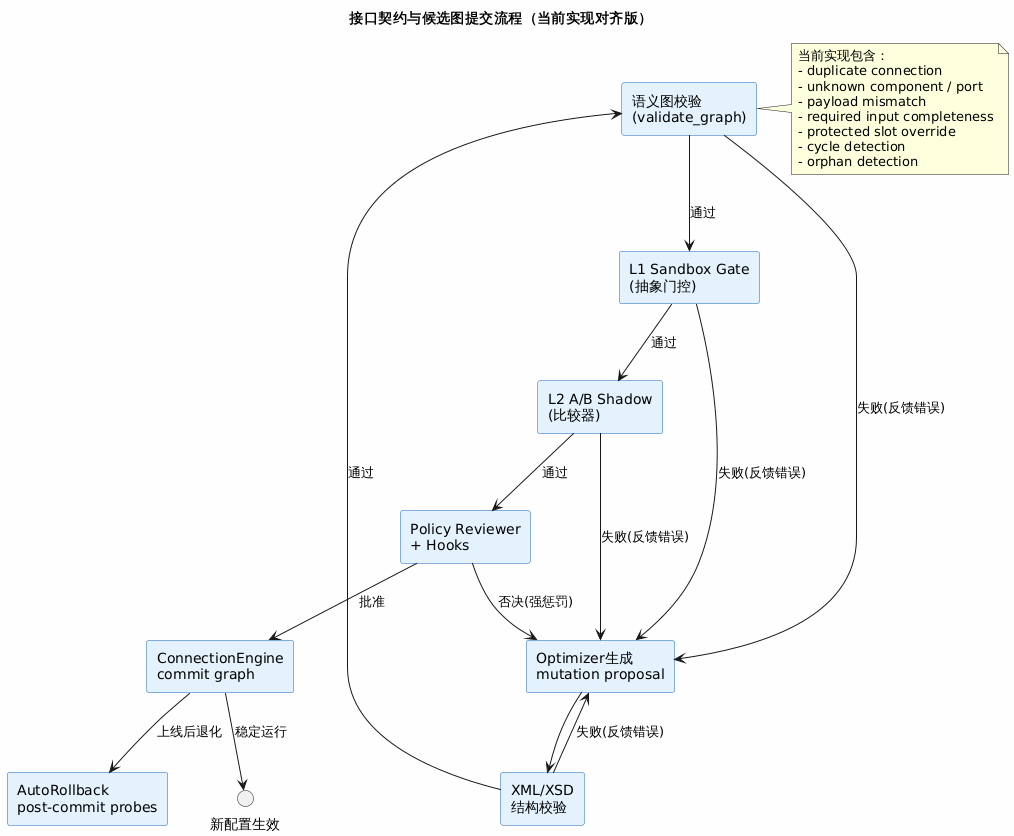
\includegraphics[width=0.85\textwidth]{assets/fig3_interface_contract.png}
\caption{接口契约与配置热加载流程}
\label{fig:interface_contract}
\end{figure}

\subsection{热加载状态迁移协议}

配置热加载在工程上不能理解为对 XML 文件的简单替换，因为组件内部往往持有上下文缓存、会话队列、统计计数器或中间执行状态。如果只完成结构切换而不处理状态连续性，新的组件图即使通过接口校验，也可能在恢复运行后出现上下文丢失、消息错序或行为突变。

因此，元Harness 应采用 \textbf{Suspend-Transform-Resume} 三阶段协议。第一阶段 \textbf{Suspend} 由 Runtime 暂停旧组件的对外副作用并缓存迁移窗口内的入站消息；第二阶段 \textbf{Transform} 根据新旧配置差异提取旧状态并执行转换；第三阶段 \textbf{Resume} 将转换后的状态注入新组件实例，再恢复消息投递与正常执行。整个过程应由 Runtime 以原子方式编排，以便在转换失败时直接回退到旧配置。

形式化地，若旧状态空间为 $S_{old}$，配置增量为 $\Delta P$，新状态空间为 $S_{new}$，则状态迁移可表示为映射
\[
\tau: S_{old} \times \Delta P \to S_{new}
\]
其中 $\Delta P$ 描述本轮热加载引入的参数、连接或组件结构变化。该映射强调：热加载不仅是配置变更，也是状态表示的受约束重解释。

据此，凡由 Optimizer 生成的配置变更，原则上都应携带对应的 Python 状态转换逻辑，用于把旧组件实例中的关键运行态映射到新实例。只有同时具备“配置差异”与“状态变换”两部分描述，热加载才能从静态重装升级为可控的在线迁移。

\section{本章小结}

本章详细介绍了元Harness框架的总体设计。首先阐述了借鉴 PDE 迭代收敛思想的设计理念，并说明了这一类比的适用边界；随后建立了统一术语基线（slots、contracts、candidate graph、active graph version、staged lifecycle、protected components 等），为后续章节提供一致的语义基础；接着给出了\textbf{九大核心基础组件}加\textbf{元层优化器（Optimizer）}的定义与典型组合规则，并将 Identity、Sandbox、Browser 明确归为扩展能力而非核心分类；系统描述了基于 XML 的结构化配置方案，包括 \texttt{<Component>}、\texttt{<Connection>}、\texttt{<MetaCycle>} 和 \texttt{<Sandbox>} 四类核心标签；重点论述了接口契约的必要性、兼容性校验的五条规则、契约驱动的动作空间剪枝、候选图组装与版本管理、组件分阶段生命周期、五条设计约束，以及配置热加载中的 STR（Suspend-Transform-Resume）状态迁移协议。这些设计共同构成了元Harness系统安全、灵活、可扩展的运行时基础。
